
\documentclass{ppgeesa}

%%%%%%%%%%%%%%%%%%%%%%%%%%%%%%%%%%%%%%%%%%%%%%%%%%%%%%%%%%%%%%%%%%%%%%%%%%%%%%%%%%%%%%%%%%%%%%%%%%%%%%%%%%%%%%%%%

\usepackage[latin1]{inputenc}
\usepackage{graphicx}
\usepackage{hyperref}
\usepackage{tikz}
\usepackage{amsmath}
\usepackage{listings}

\lstset{stepnumber=2, frame=single,tabsize=2, breaklines=true, basicstyle=\footnotesize}

\hypersetup{
	colorlinks,
	debug=true,
	linkcolor=black,  %%% cor do tableofcontents, \ref, \footnote, etc
	citecolor=red,  %%% cor do \cite
	urlcolor=blue,   %%% cor do \url e \href
	bookmarksopen=true,
	pdftitle={Modelagem e identifica��o de sistemas},
	pdfauthor={Tassiano Neuhaus},
	pdfsubject={M�todos n�o param�tricos de identifica��o},
	pdfkeywords={Identifica��o de sistemas}
	%pdfpagemode=FullScreen
}

%%%%%%%%%%%%%%%%%%%%%%%%%%%%%%%%%%%%%%%%%%%%%%%%%%%%%%%%%%%%%%%%%%%%%%%%%%%%%%%%%%%%%%%%%%%%%%%%%%%%%%%%%%%%%%%%%


\begin{document}

\title{M�todos n�o param�tricos de identifica��o de sistemas}

\author{Tassiano Neuhaus\\
{\small Universidade Federal do Rio Grande do Sul - Departamento de Engenharia El�trica\\Av. Osvaldo Aranha, 103 - Bairro Bom Fim CEP: 90035-190 - Porto Alegre - RS - Brasil}\\
}%\thanks{Tassiano Neuhaus, tassianors@gmail.com, tel +55-51-91760154}}

\maketitle
\thispagestyle{empty}\pagestyle{empty}

\begin{abstract}
Neste trabalho ser� apresentado a caracteriza��o de um sistema sujeito a incertezas. A caracteriza��o
ser� baseada nos seguintes tipos: Polit�picas, limitadas em norma, diagonal e elemento por elemento.

Para cada uma das incertezas caracterizadas ser� projetada uma realimenta��o de estados para minimizar
a norma {\it{$H_2$}} em malha fechada. O mesmo ser� feito para minimizar a norma {\it{$H_{\infty}$}}

Ao fim ser� feita uma breve compara��o entre os resultados obtidos no trabalho.
\end{abstract}

\begin{IEEEkeywords}
Identifica��o de sistemas lineares, m�todos n�o param�tricos.
\end{IEEEkeywords}

%===============================================================================
\section{Introdu��o}

Neste trabalho ser� apresentado o projeto de controladores denominados Robustos. Para 
tanto ser� apresentado o conceito de um controlador Robusto. A fim de modelar um
sistema sujeito a incertezas ser� apresentado alguns m�todos para que sua modelagem
matem�tica seja poss�vel. 

Para tornar o estudo mais claro ser� utilizado um sistema f�sico onde estar� sujeito a
perturba��es e/ou incertezas. Sobre este sistema ser� feito a modelagem seguindo cada um
dos processos e com estes modelos ser� efetuado uma simula��o. 

Esta simula��o ser� baseada no projeto de uma realimenta��o de estados com o intuito de
satisfazer a minimiza��o da norma $H2$ e $H_{\infty}$.

O sistema utilizado � apresentado no sistema de equa��es de estado descrito em (\ref{eq:intro_sis}).

\begin{equation}
\begin{matrix}
A=\begin{bmatrix}
0 & 1\\ 
-ba &a+b 
\end{bmatrix} &
B=\begin{bmatrix}
0\\ 
k
\end{bmatrix} 
\end{matrix}
\label{eq:intro_sis}
\end{equation}

Este sistema possui a fun��o de transfer�ncia apresentado em (\ref{eq:intro_transf}).

\begin{equation}
G(s)=\frac{k}{(s-a)(s-b)}
\label{eq:intro_transf}
\end{equation}

Os par�metros $a, b, k$ est�o sujeitos as varia��es apresentadas em (\ref{eq:intro_limit}).

\begin{equation}
\begin{matrix}
b= & -0.012725 & \\ 
k= & [k_1 \; k_2] =& [-0.4649.10^{-4} \; -0.7449.10^{-4}]\\ 
a= & [a_1 \; a_2] =& [-0.25 \; -2]
\end{matrix}
\label{eq:intro_limit}
\end{equation}


\section{Bode e Nyquist}
\label{sec:bode_nyquist}
%===============================================================================

Nesta sec�o ser� apresentado o diagrama de Bode e Nyquist para o processo, descrito 
em (\ref{fig:system}). Utilizando-se duas abordagens: 

\begin{itemize}
\item Basico onde aplica-se um onda senoidal na entrada do processo e mede-se a amplitude
e a fase da onda que foi produzida na sa�da.

\item M�todo melhorado, onde tenta-se reduzir a influ�ncia do ruido sobre as medidas coletadas.

\end{itemize}

A fim de comparar os resultados obtidos com um resultado correto, foi apresentado nas
Figuras (\ref{fig:bode_sem_ruido}) e  (\ref{fig:nyquist_sem_ruido}) os diagramas de 
Bode e Nyquist respectivamente do sistema sem ruido. Nas abordagens seguintes o sistema 
considerado ter� ruido e ser� feito um comparativo para determinar qual m�todo se aproxima
mais da resposta real do sistema.

\begin{figure}[htbp]
	\center
	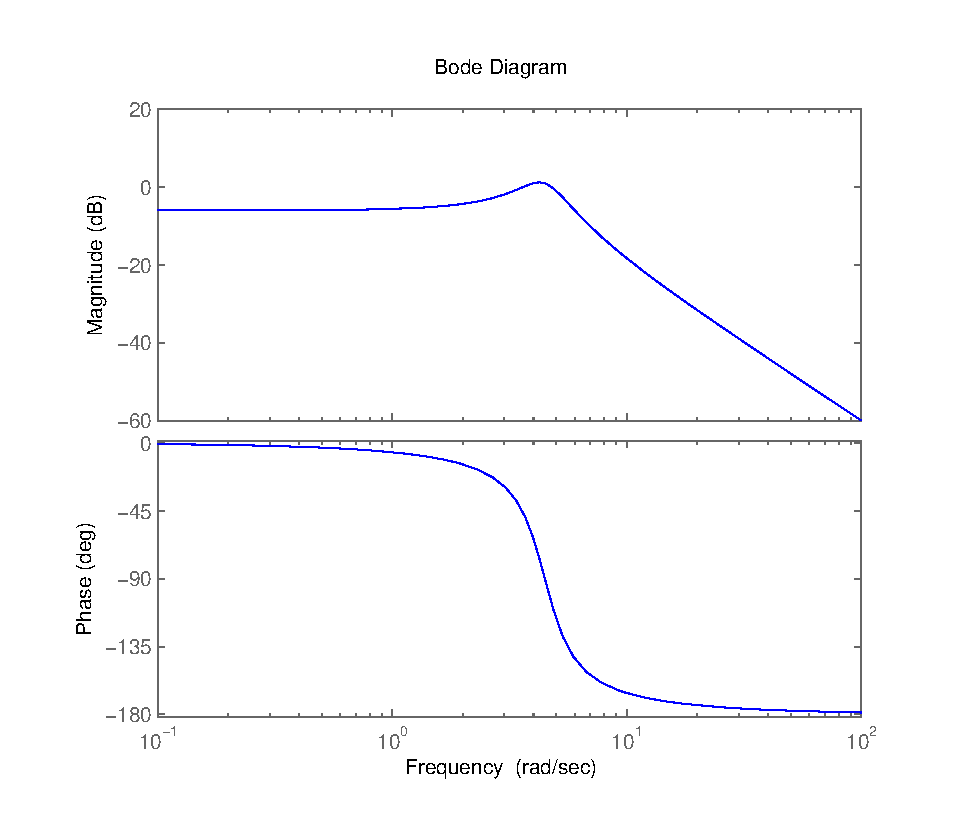
\includegraphics[width=0.98\columnwidth]{figures/bode_sem_ruido.eps}
	\caption{Diagrama de bode do sistema sem ruido.}
	\label{fig:bode_sem_ruido}
\end{figure}

\begin{figure}[htbp]
	\center
	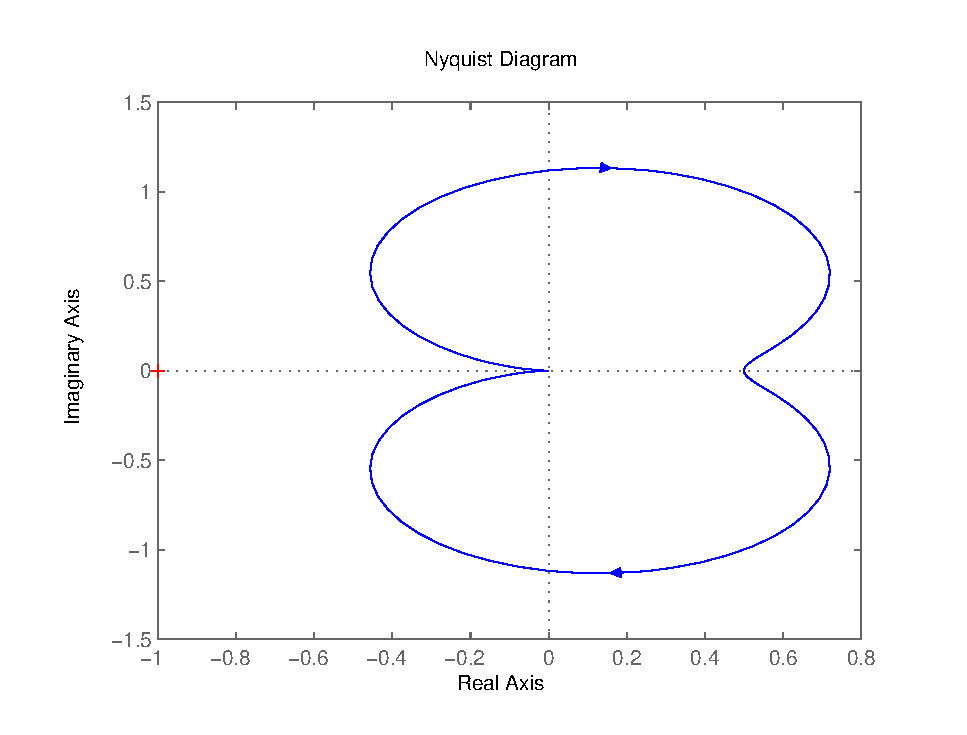
\includegraphics[width=0.98\columnwidth]{figures/nyquist_sem_ruido.eps}
	\caption{Diagrama de Nyquist do sistema sem ruido.}
	\label{fig:nyquist_sem_ruido}
\end{figure}

%===============================================================================
\subsection{M�todo B�sico}
\label{sec:bode_nyquest_basico}

Este m�todo simples consiste em aplicar uma onda senoidal na entrada do processo e observar qual
� a defasagem que a planta imp�em sobre a onde da entrada e a qual � o ganho de amplitude que 
� aplicado.

Como a planta em quest�o possui ru�do aditivo na sa�da, tem-se que as medidas efetuadas por este
m�todo s�o muito imprecisas, para calcular a amplitude do sinal de saida, basta analisar um ponto
que fique mediano ao ruido observado, mas para a fase, esta informa��o � mais complicada, pois como
a defasagem na planta em estudo � pequena, o ruido � muito grande, proporcionalmente, tornando as
medidas muito incertas.

Na Figura (\ref{fig:basic_method_1}) apresenta-se uma resposta padr�o para uma entrada senoidal.
Observa-se que a sa�da possui um ruido significante. Utilizando-se o mesmo procedimento, para diversas
frequencias de ondas senoidais na entrada do processo, obtem-se diversos pontos do diagrama de 
resposta em frequencia do processo.

\begin{figure}[htbp]
	\center
	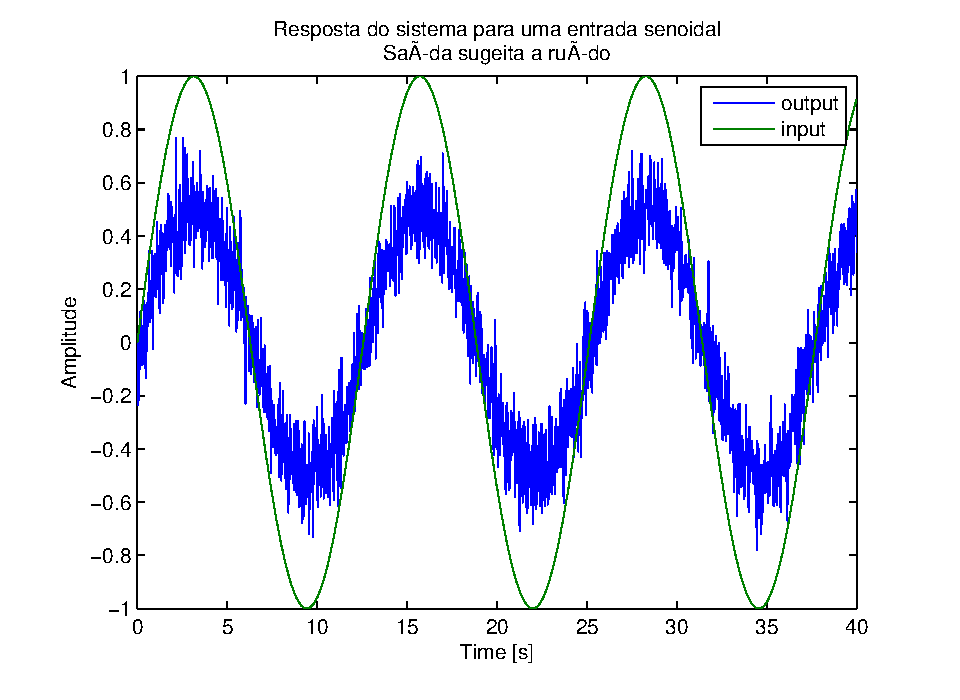
\includegraphics[width=0.98\columnwidth]{figures/basic_method_1.eps}
	\caption{Resposta do sistema para entrada senoidal}
	\label{fig:basic_method_1}
\end{figure}

Esta informac�es coletadas sobre o ganho e o deslocamento de fase aplicado sobre o sistema, chega-se as
informa��es que estao contidas na Tabela (\ref{tab:basic_method})

\begin{table}[htbp]
  \begin{center}
	\caption{M�todo b�sico}
	\label{tab:basic_method}
	\begin{small}
	  \begin{tabular}{cll}
		\hline
		Frequ�ncia			& Ganho			& Fase [deg]	\\
		\hline
		0.1					& 				& 				\\
		0.1					& 				& 				\\
		0.1					& 				& 				\\
		0.1					& 				& 				\\
		0.1					& 				& 				\\
		0.1					& 				& 				\\
		0.1					& 				& 				\\
		0.1					& 				& 				\\
		0.1					& 				& 				\\
		0.1					& 				& 				\\
		\hline
	  \end{tabular}
	\end{small}
  \end{center}
\end{table}

%===============================================================================
\subsection{M�todo melhorado}
\label{sec:bode_nyquest_melhorado}


\section{Resposta impulsiva}
\label{sec:resp_impulse}
%===============================================================================

A resposta impulsiva de um sistema consegue caracterizar por completo o comportamento de um
sistema para qualquer tipo de entrada. Pois convoluindo-se no tempo esta fun��o, com o 
sinal de entrada, tem-se o sinal de sa�da do sistema.

O objetivo nesta se��o � apresentar um m�todo para estimar-se esta resposta impulsiva do sistema.

Sabe-se que a equa��o apresentada em (\ref{eq:yt_h}) � verdadeira, que apresenta a convolu��o
do sinal discreto pela resposta impulsiva do sistema, acrescido de ruido.

\begin{equation}
y(t)=\sum_{k=0}^{\infty}h(k)u(t-k)+\nu (t)
\label{eq:yt_h}
\end{equation}

Em (\ref{eq:wiener_hopf}) tem-se a equa��o de Wiener-Hopf.

\begin{equation}
r_{yu}(\tau)=\sum_{k=0}^{\infty}h(k)r_u(\tau-k)
\label{eq:wiener_hopf}
\end{equation}

A fun��o covari�ncia em (\ref{eq:wiener_hopf}) pode ser obtida pelas equa��es (\ref{eq:ryu}) e
(\ref{eq:ru}).

\begin{equation}
\hat{r}_{yu}(\tau)=\frac{1}{N}\sum_{t=1}^{N-\tau}y(t+\tau)u(t)
\label{eq:ryu}
\end{equation}

\begin{equation}
\hat{r}_{u}(\tau)=\frac{1}{N}\sum_{t=1}^{N-\tau}u(t+\tau)u(t)
\label{eq:ru}
\end{equation}

Para $\tau = 0, 1, 2 ...$ e o sistema causal (y=0, para t <0).

Aplicando-se um sinal aleat�rio da entrada do sistema, a resposta impulsiva do mesmo 
pode ser obtida por (\ref{eq:h_noise}).

\begin{equation}
h(k)=\frac{r_{yu}(k)}{r_u(0)}
\label{eq:h_noise}
\end{equation}

Utilizando o c�digo do matlab apresentado no anexo 1, obteve-se a resposta impulsiva
apresentada na Figura (\ref{fig:h_impulse}). Na figura (\ref{fig:impulse}) apresenta-se 
a resposta impulsiva do sistema sem ruido, calculado pela fun��o Impulse do matlab.

\begin{figure}[htbp]
	\center
	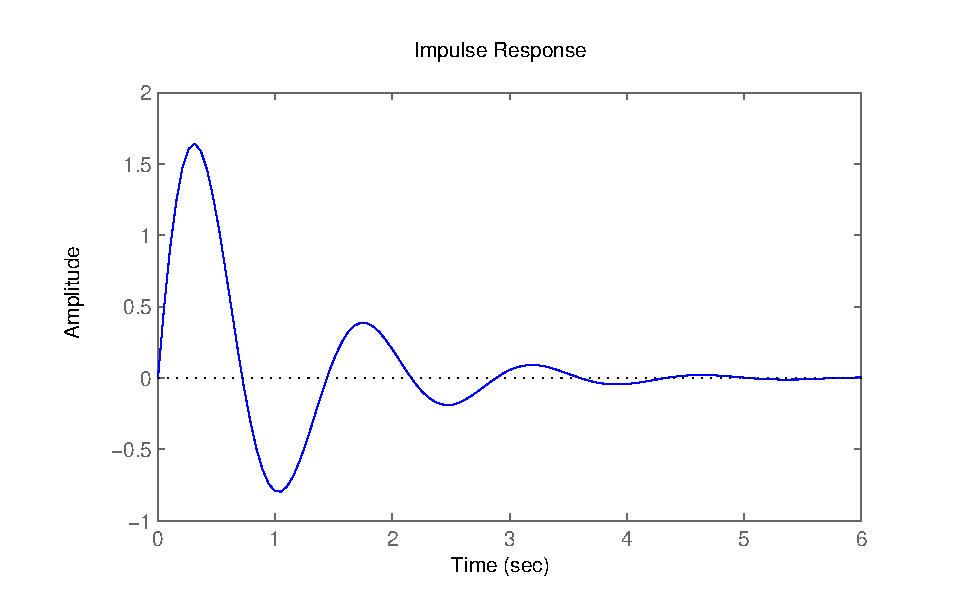
\includegraphics[width=0.98\columnwidth]{figures/impulse_sem_ruido.eps}
	\caption{Resposta impulsiva do sistema sem a interfer�ncia do ruido, obtido utilizando a
	fun��o impulse do Matlab.}
	\label{fig:impulse}
\end{figure}

\begin{figure}[htbp]
	\center
	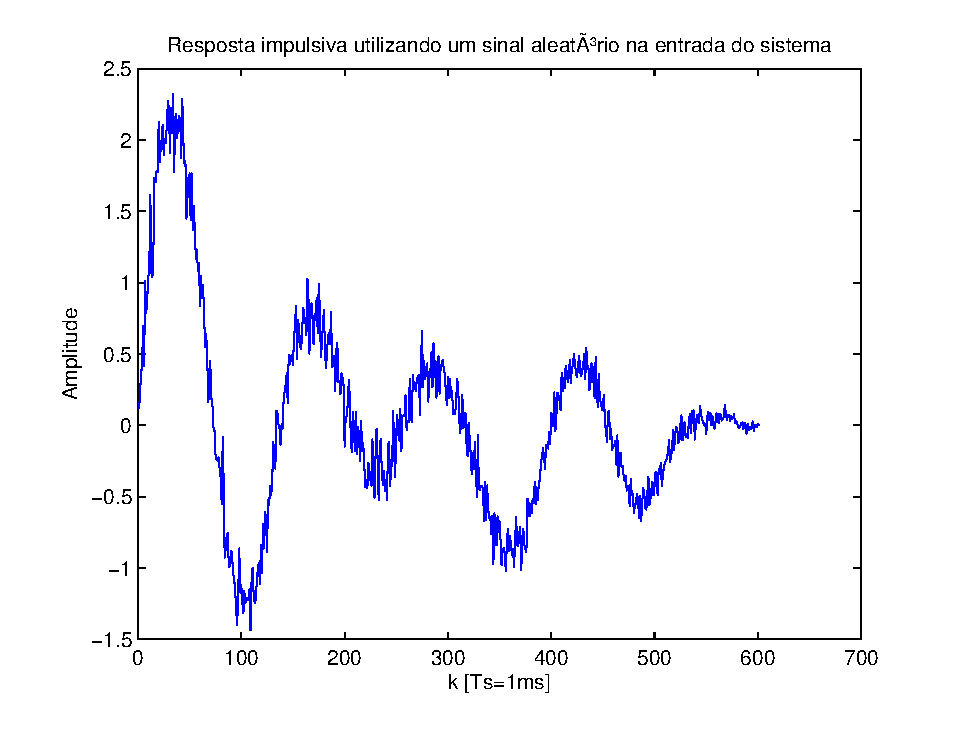
\includegraphics[width=0.98\columnwidth]{figures/impulse_com_ruido.eps}
	\caption{Resposta impulsiva do sistema com a interfer�ncia do ruido, obtido utilizando 
		um sinal aleat�rio na entrada do sistema.}
	\label{fig:h_impulse}
\end{figure}



%===============================================================================
\section{Conclus�es}
\label{sec:concl}
%===============================================================================

Neste trabalho foram apresentados dois m�todos para identifica��o de sistemas lineares,
ambos os m�todos se encontram na categoria de m�todos param�tricos de identifica��o, que 
de forma simplificada, tentam estimar os par�metros de uma fun��o de transfer�ncia que
represente o sistema f�sico em quest�o. Os m�todos utilizados foram o dos m�nimos quadrados
e das vari�veis instrumentais.

O sistema f�sico utilizado foi o controle de posi��o de um motor DC, e os dados coletados
para a identifica��o foram gerados a partir da aplica��o de sinais de refer�ncia tais como
rampas, senoides e ondas quadradas. Para cada um destes conjuntos foi obtido uma estimativa
dos par�metros do modelo utilizado.

Para efetuar a estimativa do sistema f�sico em quest�o, foi necess�rio determinar um modelo,
este foi determinado baseado no conhecimento das caracter�sticas do sistema e algumas simplifica��es 
foram efetuadas, a fim de tornar o modelo matem�tico o mais simples poss�vel, mas que ainda 
consiga descrever o sistema dentro de uma margem aceit�vel de precis�o.

O m�todo dos m�nimos quadrados (\ref{sec:mmq}) obteve resultados para a estimativa dos par�metros
que podem ser encontrados na Tabela (\ref{tab:mmq_results}). Houveram pequenas diverg�ncias nos 
par�metros entre um conjunto de dados e outro, o que n�o � desej�vel, isso pode ser devido a
imprecis�es do modelo utilizado, (pode ser devido as simplifica��es do modelo, ou de din�micas n�o
levadas em considera��o).

O m�todo das vari�veis instrumentais (\ref{sec:iv}) obteve resultados semelhantes ao m�todo 
dos m�nimos quadrados, mas com valores mais pr�ximos nos diferentes grupos de medidas. Os 
resultados para este m�todo foram apresentados na Tabela (\ref{tab:iv_results}).

De forma geral este trabalho abordou e demonstrou como � o procedimento e no que se baseiam 
dois m�todos de identifica��o de sistemas lineares sujeitos a incertezas, perturba��es e 
ru�dos. N�o � o objetivo deste trabalho detalhar esmiu�ar a matem�tica destes m�todos e
sim apresentar um exemplo pr�tico, e demonstrar sua utilidade.

A aplicabilidade deste t�pico de engenharia � de uma aplicabilidade imensa, sendo muito importante 
nas mais diversas �reas a correta identifica��o de sistemas para que, a partir do conhecimento 
matem�tico de sua din�mica, possa se agir sobre este sistema, a fim de obter os resultados desejados
de forma eficiente e com propriedade sobre as a��es tomadas, uma vez que o sistema identificado
� identificado e sabe-se o qu�o boa esta aproxima��o do sistema real pode ser.


\bibliographystyle{IEEEtran}
\bibliography{biblio}

\end{document}
